
\item O tijolo de \SI{1}{\kilogram} desliza para baixo por um telhado liso de tal maneira que quando ele está em $A$ tem velocidade de \SI{1.5}{\meter/\second}. Determine a velocidade do tijolo imediatamente antes de ele deixar a superfície em $B$, a distância $d$ da parede até atingir o solo e a velocidade com a qual ele bate no solo.

\import{answers/}{answer-2}

\vspace{-2.3cm}
\begin{flushright}
    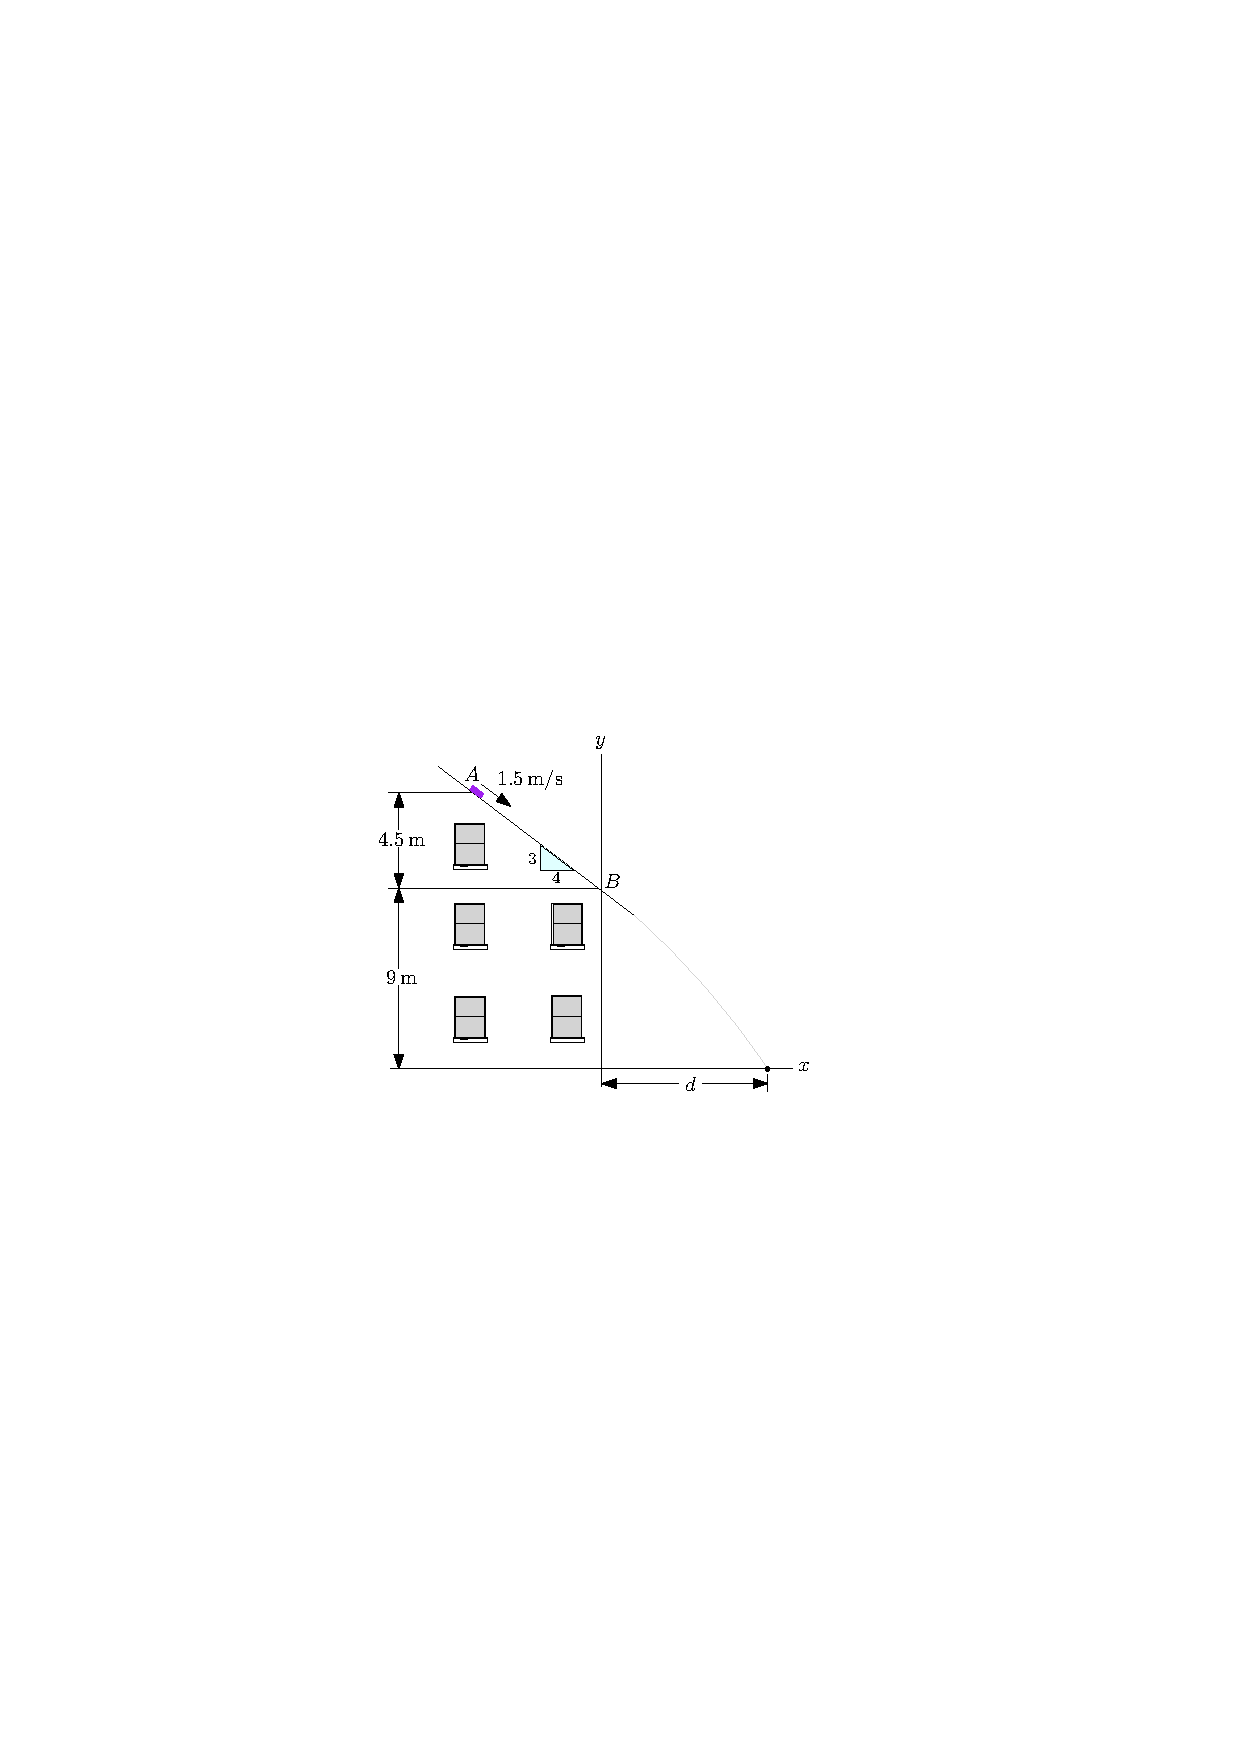
\includegraphics[scale=1.2]{images/draw_2.pdf}
\end{flushright}
